%%%%%%%%%%%%%%%%%%%%%%%%%%%%%%%%%%%%%%%%%%%%%%%%%%%%%%%%%%%%%%%%%%%%%%%%
%
%   SMT-COMP 2023 - Futur of SMTCOMP without starexec
%
%   1 hour
%
%%%%%%%%%%%%%%%%%%%%%%%%%%%%%%%%%%%%%%%%%%%%%%%%%%%%%%%%%%%%%%%%%%%%%%%%

\documentclass[table]{beamer}
\usepackage[utf8]{inputenc}
\usepackage{xcolor}
\usepackage{tikz}
\usetikzlibrary{shapes,shapes.callouts,automata,trees}
\usetikzlibrary{decorations.pathmorphing,external,fit}
\usetikzlibrary{calc}
\usetikzlibrary{backgrounds} %used for the CEGAR figure
\usepackage{amssymb}
\usepackage{clrscode}
\usepackage{pifont}
\usepackage{pdfpages}
\usepackage{graphicx}
\usepackage{listings}
\geometry{papersize={16cm,9cm}}
%\tikzexternalize

\colorlet{MYred}{red!70!black}
\definecolor{MYgreen}{rgb}{.1,.5,0}
\definecolor{MYblue}{rgb}{0,.42,.714}
\colorlet{MYgray}{white!95!MYblue}
\colorlet{MYorange}{orange!80!black}
\definecolor{gold}{rgb}{.8,.6,0}
\colorlet{silver}{white!55!black}
\colorlet{bronze}{brown!70!black}
\def\tick{\ding{52}}
\def\cross{\ding{54}}

%%%%%%%%%%%%%%%%%%%%
%%% Beamer stuff %%%
%%%%%%%%%%%%%%%%%%%%
\usetheme{default}
\useinnertheme{rounded}
\setbeamertemplate{frametitle}[default][center]
\setbeamertemplate{footline}{\quad\hfill\footnotesize\insertframenumber\strut\kern1em\vskip2pt}
\setbeamertemplate{navigation symbols}{}
\setbeamertemplate{itemize/enumerate subbody begin}{\normalsize}
\usefonttheme[onlymath]{serif} % Nicer formulas
\setbeamercolor{block body}{bg=black!10}
\setbeamercolor{block title}{bg=black!20}

\AtBeginSection[]{
  \begin{frame}
  \vfill
  \centering
  \begin{beamercolorbox}[sep=8pt,center,shadow=true,rounded=true]{title}
    \usebeamerfont{title}\insertsectionhead\par%
  \end{beamercolorbox}
  \vfill
  \end{frame}
}

\def\emph#1{\textcolor{MYblue}{#1}}

%%% Titel, Autor und Datum des Vortrags:
\title{Discussion on Future of SMT-COMP}
\author{Martin Bromberger \and Jochen Hoenicke \and \emph{Fran\c{c}ois Bobot}}
\date{July 5, 2023}

%% Institut
\institute{
CEA List, France \and
MPI für Informatik, Germany \and
Certora, Israel
}


%%%%%%%%%%%%%%%%%%%%%%%%%%%%%%%
% MACROS

% database symbol (from stackexchange)

\makeatletter
\tikzset{
    database/.style={
        path picture={
            \draw (0, 1.5*\database@segmentheight) circle [x radius=\database@radius,y radius=\database@aspectratio*\database@radius];
            \draw (-\database@radius, 0.5*\database@segmentheight) arc [start angle=180,end angle=360,x radius=\database@radius, y radius=\database@aspectratio*\database@radius];
            \draw (-\database@radius,-0.5*\database@segmentheight) arc [start angle=180,end angle=360,x radius=\database@radius, y radius=\database@aspectratio*\database@radius];
            \draw (-\database@radius,1.5*\database@segmentheight) -- ++(0,-3*\database@segmentheight) arc [start angle=180,end angle=360,x radius=\database@radius, y radius=\database@aspectratio*\database@radius] -- ++(0,3*\database@segmentheight);
        },
        minimum width=2*\database@radius + \pgflinewidth,
        minimum height=3*\database@segmentheight + 2*\database@aspectratio*\database@radius + \pgflinewidth,
    },
    database segment height/.store in=\database@segmentheight,
    database radius/.store in=\database@radius,
    database aspect ratio/.store in=\database@aspectratio,
    database segment height=0.1cm,
    database radius=0.25cm,
    database aspect ratio=0.35,
}
\makeatother

%%%%% json lstlisting %%%%%%%%%

\definecolor{eclipseStrings}{RGB}{42,0.0,255}
\definecolor{eclipseKeywords}{RGB}{127,0,85}
\colorlet{numb}{magenta!60!black}

\lstdefinelanguage{json}{
    basicstyle=\normalfont\ttfamily,
    commentstyle=\color{eclipseStrings}, % style of comment
    stringstyle=\color{eclipseKeywords}, % style of strings
 %   numbers=left,
    numberstyle=\scriptsize,
    stepnumber=1,
    numbersep=8pt,
    showstringspaces=false,
    breaklines=true,
    frame=lines,
%    backgroundcolor=\color{gray}, %only if you like
    string=[s]{"}{"},
    comment=[l]{:\ "},
    morecomment=[l]{:"},
    literate=
        *{0}{{{\color{numb}0}}}{1}
         {1}{{{\color{numb}1}}}{1}
         {2}{{{\color{numb}2}}}{1}
         {3}{{{\color{numb}3}}}{1}
         {4}{{{\color{numb}4}}}{1}
         {5}{{{\color{numb}5}}}{1}
         {6}{{{\color{numb}6}}}{1}
         {7}{{{\color{numb}7}}}{1}
         {8}{{{\color{numb}8}}}{1}
         {9}{{{\color{numb}9}}}{1}
}

%%%%%%%%%%%%%%%%%%%%%%%%%%%%%%%

\newcommand\vitem{\vfill\item}

\begin{document}

\begin{frame}
  \titlepage
\end{frame}

\newcommand{\mylogo}[1]{\includegraphics[height=1.5em]{#1}}

\newbox{\logostarexec}
\savebox{\logostarexec}{\mylogo{starlogo.png}}

\newcommand{\logolaptop}{\mylogo{512px-OOjs_UI_icon_laptop-progressive.svg.png}}

\begin{frame}
    \frametitle{Current infrastructure}
    \pause
    \begin{tabular}{cl}
        \mylogo{iowa_university.png}\usebox{\logostarexec} & Benchmark uploaded to StarExec from Iowa Gitlab \\\pause
        \mylogo{Google__G__Logo.svg.png} & Applications through Google form \\\pause
        \usebox{\logostarexec} & Solvers are uploaded to StarExec \\\pause
        \mylogo{You've_got_mail.png} & Modification of the applications handled by mail \\\pause
        \logolaptop & Solvers downloaded, wrapped locally, uploaded to StarExec \\\pause
        \logolaptop & Benchmark selection and job created locally \\\pause
        \usebox{\logostarexec} & Jobs sent to StarExec and run \\\pause
        \usebox{\logostarexec} & Download results from StarExec \\\pause
        \logolaptop \usebox{\logostarexec} & Fix benchmark selection, add fixed
         version of the solvers, run jobs on Starexec \\\pause
        \logolaptop & Score the results, generate data for the website \\
    \end{tabular}
\end{frame}

\newcommand{\onlystarexec}{\only<1>{\usebox{\logostarexec}}}
\newcommand{\onlylaptop}{\only<1-4>{\logolaptop}}
\newcommand{\logocloud}{\mylogo{1280px-Amazon_Web_Services_Logo.svg.png}
\mylogo{Google-Cloud-Emblem.png}
\mylogo{Microsoft-Azure.png}}
\newcommand{\onlycloudfirst}{\only<4->{\logocloud}}
\newcommand{\onlycloudsecond}{\only<5->{\logocloud}}
\newcommand{\logogithub}{\mylogo{free-github-163-761603.png}}
\newcommand{\logozenodo}{\mylogo{zenodo.png}}

\frame<1>[label=summary]{
    \frametitle{Needed infrastructure}
    \begin{itemize}
        \item Store benchmark : \mylogo{iowa_university.png}\onlystarexec %iowa and starexec
        \item Participants registration : \only<-4>{\mylogo{Google__G__Logo.svg.png}\mylogo{You've_got_mail.png}}
        \only<5->{\logogithub}
        %google and starexec
        \item Select the benchmarks: \onlylaptop\onlycloudsecond
        \item Run the jobs : \onlystarexec\onlycloudfirst%starexec
        \item Store the datas : \onlystarexec\onlycloudfirst%starexec
        \item Archive the datas : \onlystarexec\only<3->{\logozenodo}%starexec
%        \item Store the raw results (sq csv 148Mo, 16Mo compressed) : \usebox{\logostarexec}%starexec
%        \item Store the artifacts (mv Go proof Go) : \usebox{\logostarexec} %starexec
        \item Run scoring script and generate website : \onlylaptop\onlycloudsecond\logogithub%localy and github
    \end{itemize}
}

\begin{frame}
    \frametitle{StarExec}
    Since 2013, StarExec has run 80 competitions and events across its 16 registered communities(SAT, TPTP, Termination,...).  
    StarExec is supported by a \$1.85 million USD grant (NSF)

%Several people have contributed in various capacities to the StarExec project
%so far.
\vfill
Shepherded by Aaron Stump
\vfill
Involved in the development: {\small Eric Burns, Todd Elvers,
Albert Giegerich, Pat Hawks, Tyler Jensen, Wyatt Kaiser, Ben McCune, Muhammad
Nassar, CJ Palmer, Vivek Sardeshmukh, Skylar Stark, and Ruoyu Zhang.}
\vfill
Computer system support and assistance: {\small Hugh Brown, Dan Holstad, Jamie
Tisdale, and JJ Ulrich}

%In addition to the members of the Advisory Board, the following people have
%provided useful feedback and input: Clark Barrett, Christoph Benzmüller, Armin
%Biere, David Cok, Morgan Deters, Jürgen Giesl, Alberto Griggio, Thomas
%Krennwallner, Jens Otten, Andrei Paskevich, Olivier Roussel, Martina Seidl,
%Stephan Schulz, Michael Tautschnig, Christoph Wintersteiger, and Harald Zankl.
\end{frame}

\begin{frame}
    \frametitle{StarExec: job pairs}
\begin{center}
    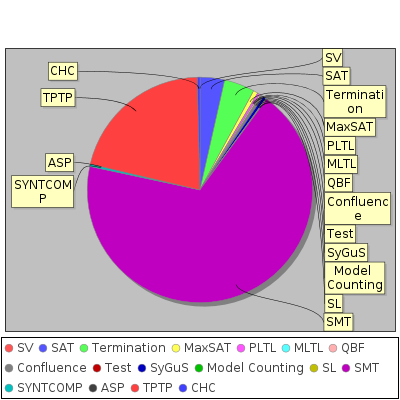
\includegraphics[width=\textwidth,height=\textheight,keepaspectratio]{statistics_starexec.png}    
\end{center}

\end{frame}
\begin{frame}
    \frametitle{StarExec is closing}

    \begin{center}
        
        \huge{Decommissioned starting August 2024}
    \end{center}

\end{frame}

\againframe<2>{summary}

\begin{frame}
    \frametitle{Archive: Past results and Artifacts}

    \begin{itemize}
        \item Solvers
        \item Raw results
        \item Solver output 
    \end{itemize}
    \vfill
    \pause
    \logozenodo: EC funded research. Leveraging CERN developed tools for Big Data management and extended Digital Library capabilities for Open Data
    \begin{itemize}
        \item Open
        \item Max 50 GB per dataset
        \item DOI
    \end{itemize}
\vfill
    NB: StarExec should do the upload (because downloading from StarExec is very slow)

\end{frame}

\againframe<3>{summary}


% \begin{frame}
%     \frametitle{Future competition}

% \begin{itemize}
%     \item CPU
%     \item Intermediate Data-storage
%     \item Permanent Data-storage (like past competition)
% \end{itemize}

% \end{frame}



\begin{frame}
    \frametitle{Future competitions: Cloud? \logocloud}
\begin{columns}
    \column{0.5\textwidth}
    Slurm (open-source job scheduler):
    \begin{itemize}
        \item Available in cloud providers
        \item Could be available in academic clusters
        \item Allows to do the selection in the cloud
    \end{itemize}
    \column{0.5\textwidth}
    Batch
    \begin{itemize}
        \item Each provider as its own API 
        \item Simpler
        \item e.g. \url{https://github.com/Z3Prover/PerformanceTest}
    \end{itemize}
\end{columns}
    \pause
    \vfill
    \begin{center}
        \large
        Who already used cloud for benchmarking?
    \end{center}
\end{frame}


\againframe<4>{summary}

\begin{frame}
    \frametitle{Participant registration}
    Github MR with \lstinline{bub4.json}:
    
    \lstinputlisting[language=json]{prover.json}
\end{frame}

\againframe<5>{summary}

\begin{frame}
    \frametitle{Other simplifications}
    \begin{itemize}
        \item Currently 3 repositories $\implies$ 1 repository
        \item Bash, sed, awk, python $\implies$ python
    \end{itemize}
\pause
\vfill
    \begin{center}
        {\large Is the secrecy of the result important to keep?}
    \end{center}
\end{frame}

\begin{frame}
    \frametitle{Questions?}

    \begin{itemize}
        \item Zenodo? For longterm archive
        \item Reproducibility of the result?
        \item Experience with cloud computing?
        \item Need for sponsorship
    \end{itemize}
\end{frame}

\end{document}
